
\section{Wemos Lolin32 Lite}

The Wemos LOLIN32 Lite is a low-cost, low-power system on a chip (SoC)  microcontroller that is popular for Internet of Things (IoT) projects. It is based on the ESP32 SoC, which has a 32-bit dual-core processor, 4MB of flash memory, and 520kB of RAM. The LOLIN32 Lite also has Wi-Fi and Bluetooth connectivity, making it ideal for this projects for sending and receiving data to and from Digital Twin through a wireless connection.


% \begin{figure}[H]    
%     \caption{}
%     % \centring
%     \begin{subfigure}[b]{0.45\textwidth}
%     \caption{Number of selected papers per publisher.}
       
        
%     \end{subfigure}
%     \begin{subfigure}[b]{0.45\textwidth}
%     \caption{Number of selected papers per source.}
       
%     \end{subfigure}
%     \label{fig:esp32}
% \end{figure}



\begin{figure}[ht]
  \centering
  \begin{minipage}{0.5\textwidth}
    \centering
    \caption{Temporary Image Replacement for ESP32 board}
    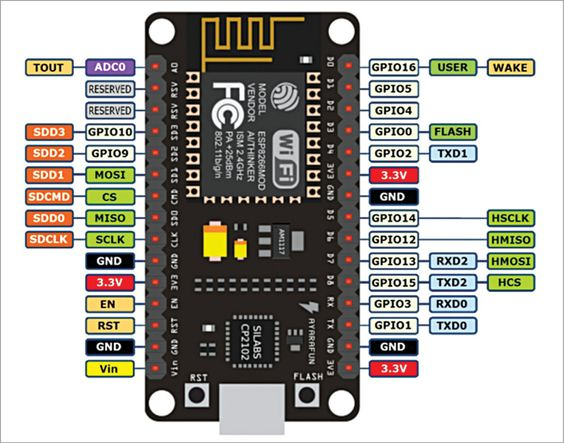
\includegraphics[width=\textwidth]{images/fp/ESP32.jpg}
    \label{fig:example-image}
  \end{minipage}%
  \hspace{0.2cm}
  \begin{minipage}{0.45\textwidth}
    \centering
    \begin{table}[H]
        % \tiny
        \centering
        \caption{\label{tbl:esp-spec} Technical Specification of Wemos Lolin32 Lite}
        % \resizebox{\linewidth}{!}{
        \begin{NiceTabular}{|p{2.5cm}|p{3cm}|}
        \CodeBefore
        % \rowcolors[gray]{2}{0.8}{}[cols=1-2,restart]
        \Body
        \toprule
        	Operating voltage &  3.3V \\
            \hline
        	Supported Battery &	Lipo 3.7V\\
            \hline
        	Battery Connector & PH-2 2.0mm\\
            \hline
        	Digital I/O Pins & 22 \\
            \hline
        	 RAM Memory &  512KB\\
            \hline
            Clock Speed(Max) &	240MHz \\
            \hline
            SPI Flash &	4M Bytes \\
            \hline
            Size & 57*25.4mm \\
        \bottomrule
        \end{NiceTabular}
        % }
    \end{table}
  \end{minipage}
\end{figure}

One of the key advantages of the Wemos LoLin32 Lite board is that it is supported by both the Arduino and ESP-IDF (Espressif IoT Development Framework) development environments. For our research project, we opted to use the Arduino embedded development framework in order to implement the ASCON and AES-GCM algorithms using the C and C++ programming languages. In addition, we utilized PlatformIO, an open-source platform for embedded development, to facilitate the building and deployment of our program onto the Wemos LoLin32 Lite board via the serial port.